%%%---PREAMBLE---%%%%%%%%%%%%%%%%%%%%%%%%%%%%
\documentclass[oneside,12pt,final]{sty/ucthesis-CA2012}
\pdfoutput=1

%--- Packages ---------------------------------------------------------
\usepackage[lofdepth,lotdepth,caption=false]{subfig}
\usepackage{fancyhdr}
\usepackage{hyperref}
\usepackage{amsmath, amssymb, graphicx}
\usepackage{xspace}
\usepackage{braket}
\usepackage{color}
\usepackage{setspace}
%\usepackage{subfigure} (Subfigure package clashes with another package)

%---New Definitions and Commands------------------------------------------------------
\def\p{\partial}
\def\im{\mrm{im}}
\def\Tr{\mrm{Tr}}
\def\Z{\mbb{Z}}
\def\R{\mbb{R}}
\def\C{\mbb{C}}
\def\half{\frac{1}{2}}
\def\filler{\phantom{fillerfillerfiller}}
\newcommand{\be}{\begin{equation}}
\newcommand{\ee}{\end{equation}}
\newcommand{\mbb}[1]{\mathbb{#1}}
\newcommand{\mrm}[1]{\mathrm{#1}}
\newcommand{\mcal}[1]{\mathcal{#1}}
\newcommand{\mbf}[1]{\mathbf{#1}}
\newcommand{\ph}[1]{\phantom{#1}}
\newcommand{\udten}[3]{#1^{#2}_{\ph{#2}#3}}
\newcommand{\duten}[3]{#1^{\ph{#2}#3}_{#2}}
\newcommand{\pd}[2]{\frac{\p#1}{\p#2}}
\newcommand{\D}[2]{\frac{d#1}{d#2}}

%---Set Margins ------------------------------------------------------
\setlength\oddsidemargin{0.25 in} \setlength\evensidemargin{0.25 in} \setlength\textwidth{6.25 in} \setlength\textheight{8.50 in}
\setlength\footskip{0.25 in} \setlength\topmargin{0 in} \setlength\headheight{0.25 in} \setlength\headsep{0.25 in}

%%%---DOCUMENT---%%%%%%%%%%%%%%%%%%%%%%%%%%%%
\begin{document}

%=== Preliminary Pages ============================================
\begin{frontmatter}
	%%%%%%%%%%%%%%%%%%%%%%%%%%%
% TITLE PAGE INFORMATION %
%%%%%%%%%%%%%%%%%%%%%%%%%%%


\title{A Search for $R$-parity violating supersymmetry at the 13 TeV LHC}

\author{Rohan Bhandari}

%%%%%%%%%%%%%%%%%%%%%%%%%%%%%%%%%%
% DECLARATIONS FOR FRONT MATTER %
%%%%%%%%%%%%%%%%%%%%%%%%%%%%%%%%%%
\report{Dissertation} \degree{Doctor of Philosophy} \degreemonth{June} \degreeyear{2018}
\defensemonth{May}
\defenseyear{2018}

\chair{Professor David Stuart} \othermemberA{Professor Harry Nelson} \othermemberB{Professor Nathaniel Craig}   \numberofmembers{3}

\field{Physics}
\campus{Santa Barbara}


%\title{{ University of California \\ Santa Barbara} \linebreak \\  Ph.D. Dissertation}
%\author{Tom\'as Andrade}
%\date{2012}

	\maketitle
	\approvalpage
	\copyrightpage
	\begin{dedication}

\bigskip

${}$ \\

\bigskip

${}$ \\

\bigskip

${}$ \\

\bigskip

\begin{center}
\begin{Large}
To my parents, Ramesh and Savita
\end{Large}
\end{center}


\end{dedication} 
%comment out if you don't want a dedication
	\begin{acknowledgements}

Since my childhood, I have always been fascinated by big questions about the universe, and I feel blessed to have had the opportunity to immerse myself in them for the past five years.
This dissertation encapsulates my career as a particle physicist and my contribution to answering those universal questions.
I, however, could not have done this without many helping hands to whom I owe a great deal.

First, I must thank the RichStu group---my HEX family. 
In particular, I want to thank my advisor, David Stuart, for always being a fantastic mentor, and Jeff Richman, my de facto second advisor, for his extraordinary teaching.
There is not enough space here to properly thank you for all your guidance and wisdom.
I would not be the physicist I am today without it.
To the postdocs---Ana Ovcharova, Chris West, Jae Hyeok Yoo, Manuel Franco Sevilla, and Matt Citron---and to my fellow graduate students in arms---Adam Dishaw, Alex Dorsett, Jack Bradmiller-Feld, and Ryan Heller---it was truly a pleasure to have gone through this Ph.D. with all of you.
I could not have asked for a better group of colleagues and friends.
You made grad school fun, and I'll always have fond memories of the hour-long impromptu discussions we found ourselves in, whether we were debating physics, the news, or, far more often, color themes.

I also owe much gratitude to my parents, Ramesh and Savita, without whom none of this would be possible.
It was only through their endless love and support and countless sacrifices that I was able to pursue my dreams.
Included in this is my brother, Simit, who was always willing to make time for me and share his advice.

Finally, I would like to thank my partner, Mallorie Chase, for all her support over the last few years and for moving with me to Geneva for a year-long adventure.
I am so thankful to have met you during my time here, and I am excited to tackle our next chapter in life together.

\end{acknowledgements} 

	\begin{vitae}
\addcontentsline{toc}{chapter}{Curriculum Vitae}

\begin{vitaesection}{Education}
\vspace{-0.1cm}
\item [20XX]	Ph.D. in Physics (Expected), University of California, Santa Barbara.
\item [20XX]	M.A. in Physics, University of California, Santa Barbara.
\item [20XX]	etc
\end{vitaesection}

\textbf{Publications}

Publications.

\end{vitae}
	%
%  Abstract
%

\begin{abstract}
\addcontentsline{toc}{chapter}{Abstract}
%todo: max 350 words

Abstract text. 

%\abstractsignature
\end{abstract}



	\tableofcontents
\end{frontmatter}

\begin{mainmatter}

%---Set Headers and Footers ------------------------------------------------------
\pagestyle{fancy}
\renewcommand{\chaptermark}[1]{\markboth{{\sf #1 \hspace*{\fill} Chapter~\thechapter}}{} }
\renewcommand{\sectionmark}[1]{\markright{ {\sf Section~\thesection \hspace*{\fill} #1 }}}
\fancyhf{}

\makeatletter \if@twoside \fancyhead[LO]{\small \rightmark} \fancyhead[RE]{\small\leftmark} \else \fancyhead[LO]{\small\leftmark}
\fancyhead[RE]{\small\rightmark} \fi

\def\cleardoublepage{\clearpage\if@openright \ifodd\c@page\else
  \hbox{}
  \vspace*{\fill}
  \begin{center}
    This page intentionally left blank
  \end{center}
  \vspace{\fill}
  \thispagestyle{plain}
  \newpage
  \fi \fi}
\makeatother
\fancyfoot[c]{\textrm{\textup{\thepage}}} % page number
\fancyfoot[C]{\thepage}
\renewcommand{\headrulewidth}{0.4pt}

\fancypagestyle{plain} { \fancyhf{} \fancyfoot[C]{\thepage}
\renewcommand{\headrulewidth}{0pt}
\renewcommand{\footrulewidth}{0pt}}

%=== Introduction ============================================
\chapter{Introduction}

Cum Veteres Mechanicam (uti Author est Pappus) in verum Naturalium investigatione maximi fecerint, \& recentiores, missis formis substantialibus \& qualitatibus occultis, Ph�nomena Natur� ad leges Mathematicas revocare aggressi sint: Visum est in hoc Tractatu Mathesin excolere quatenus ea ad Philosophiam spectat. Mechanicam vero duplicem Veteres constituerunt: Rationalem qu� per Demonstrationes accurate procedit, \& Practicam. Ad practicam spectant Artes omnes Manuales, a quibus utiq; Mechanica nomen mutuata est. Cum autem Artifices parum accurate operari soleant, fit ut Mechanica omnis a Geometria ita distinguatur, ut quicquid accuratum sit ad Geometriam referatur, quicquid minus accuratum ad Mechanicam. Attamen errores non sunt Artis sed Artificum. Qui minus accurate operatur, imperfectior est Mechanicus, \& si quis accuratissime operari posset, hic foret Mechanicus omnium perfectissimus. Nam \& Linearum rectarum \& Circulorum descriptiones in quibus Geometria fundatur, ad Mechanicam pertinent. Has lineas describere Geometria non docet sed postulat. Postulat enim ut Tyro easdem accurate describere prius didicerit quam limen attingat Geometri�; dein, quomodo per has operationes Problemata solvantur, docet. Rectas \& circulos describere Problemata sunt sed non Geometrica. Ex Mechanica postulatur horum solutio, in Geometria docetur solutorum usus. Ac gloriatur Geometria quod tam paucis principiis aliunde petitis tam multa pr�stet. Fundatur igitur Geometria in praxi Mechanica, \& nihil aliud est quam Mechanic� universalis pars illa qu� artem mensurandi accurate proponit ac demonstrat. Cum autem artes Manuales in corporibus movendis pr�cipue versentur, fit ut Geometria ad magnitudinem, Mechanica ad motum vulgo reseratur. Quo sensu Mechanica rationalis erit Scientia Motuum qui ex viribus quibuscunq; resultant, \& virium qu� ad motus quoscunq; requiruntur, accurate proposita ac demonstrata. Pars h�c Mechanic� a Veteribus in Potentiis quinque ad artes manuales spectantibus exculta fuit, qui Gravitatem (cum potentia manualis non sit) vix aliter quam in ponderibus per potentias illas movendis considerarunt. Nos autem non Artibus sed Philosophi� consulentes, deq; potentiis non manualibus sed naturalibus scribentes, ea maxime tractamus qu� ad Gravitatem, levitatem, vim Elasticam, resistentiam Fluidorum \& ejusmodi vires seu attractivas seu impulsivas spectant: Et ea propter h�c nostra tanquam Philosophi� principia Mathematica proponimus. Omnis enim Philosophi� difficultas in eo versari videtur, ut a Ph�nomenis motuum investigemus vires Natur�, deinde ab his viribus demonstremus ph�nomena reliqua. Et hac spectant Propositiones generales quas Libro primo \& secundo pertractavimus. In Libro autem tertio exemplum hujus rei proposuimus per explicationem Systematis mundani. Ibi enim, ex ph�nomenis c�lestibus, per Propositiones in Libris prioribus Mathematice demonstratas, derivantur vires gravitatis quibus corpora ad Solem \& Planetas singulos tendunt. Deinde ex his viribus per Propositiones etiam Mathematicas deducuntur motus Planetarum, Cometarum, Lun� \& Maris. Utinam c�tera Natur� ph�nomena ex principiis Mechanicis eodem argumentandi genere derivare liceret. Nam multa me movent ut nonnihil suspicer ea omnia ex viribus quibusdam pendere posse, quibus corporum particul� per causas nondum cognitas vel in se mutuo impelluntur \& secundum figuras regulares coh�rent, vel ab invicem fugantur \& recedunt: quibus viribus ignotis, Philosophi hactenus Naturam frustra tentarunt. Spero autem quod vel huic Philosophandi modo, vel veriori alicui, Principia hic posita lucem aliquam pr�bebunt.

In his edendis, Vir acutissimus \& in omni literarum genere eruditissimus Edmundus Halleius operam navavit, nec solum Typothetarum Sphalmata correxit \& Schemata incidi curavit, sed etiam Author fuit ut horum editionem aggrederer. Quippe cum demonstratam a me figuram Orbium c�lestium impetraverat, rogare non destitit ut eadem cum Societate Regali communicarem, Qu� deinde hortatibus \& benignis suis auspiciis effecit ut de eadem in lucem emittenda cogitare inciperem. At postquam Motuum Lunarium in�qualitates aggressus essem, deinde etiam alia tentare c�pissem qu� ad leges mensuras Gravitatis \& aliarum virium, ad figuras a corporibus secundum datas quascunque leges attractis describendas, ad motus corporum plurium inter se, ad motus corporum in Mediis resistentibus, ad vires, densitates \& motus Mediorum, ad Orbes Cometarum \& similia spectant, editionem in aliud tempus differendam esse putavi, ut c�tera rimarer \& una in publicum darem. Qu� ad motus Lunares spectant, (imperfecta cum sint,) in Corollariis Propositionis LXVI. simul complexus sum, ne singula methodo prolixiore quam pro rei dignitate proponere, \& sigillatim demonstrare tenerer, \& seriem reliquarum Propositionum interrumpere. Nonnulla sero inventa locis minus idoneis inserere malui, quam numerum Propositionum \& citationes mutare. Ut omnia candide legantur, \& defectus, in materia tam difficili non tam reprehendantur, quam novis Lectorum conatibus investigentur, \& benigne suppleantur, enixe rogo.


\begin{section}{Permissions and Attributions}
\begin{enumerate}

\item The content of chapter 2 and appendix A is the result of a collaboration with Alice and Bob, and has previously appeared in the (Journal) (paper citation). It is reproduced here with the permission of (Institution): \url{http://}.

\end{enumerate}
\end{section}

%=== Chapter 2  ============================================
\chapter{Chapter 2 Title}
%---  Section -------------------------
\begin{section}{Section Title}

Lorem ipsum dolor sit amet, consectetur adipiscing elit. Mauris et neque massa. Fusce sit amet orci libero. Morbi venenatis quam ante, in vehicula diam. Cras in dui sem, et fermentum ligula. Sed sed tellus ut purus semper pharetra euismod nec tellus. Nullam tortor justo, tincidunt sed varius vel, rhoncus id ipsum. Sed ipsum sem, bibendum id posuere sit amet, dignissim vel odio. Integer pretium mattis metus eu porta. Sed luctus, eros eu feugiat euismod, nulla augue fringilla nisi, sed gravida sem orci ac urna.

\end{section}

%=== Chapter 3  ============================================
\chapter{Chapter 3 Title}
%---  Introduction -------------------------
\begin{section}{Section Title}

\cite{Maldacena:1997re,joesbook}. Figure \ref{fig:label}.

\begin{figure}[t]
\centerline{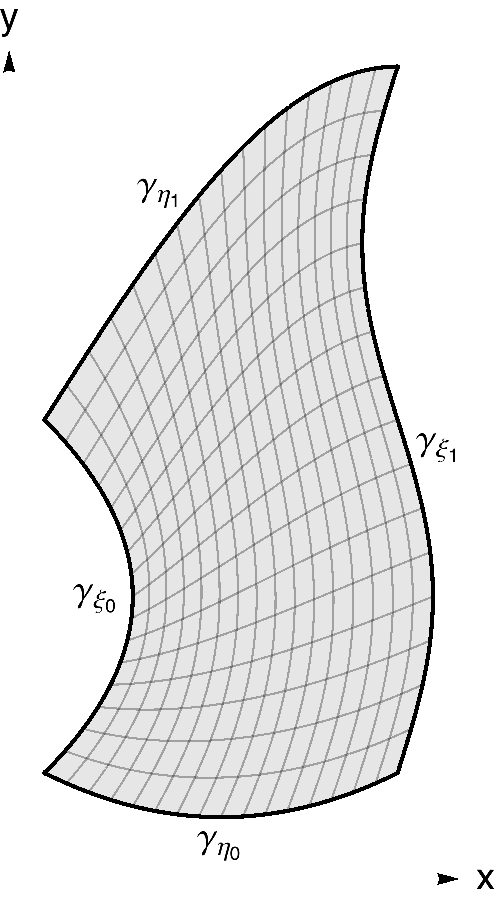
\includegraphics[width=.35\textwidth]{fig/testfig1.pdf}
\hspace{1cm}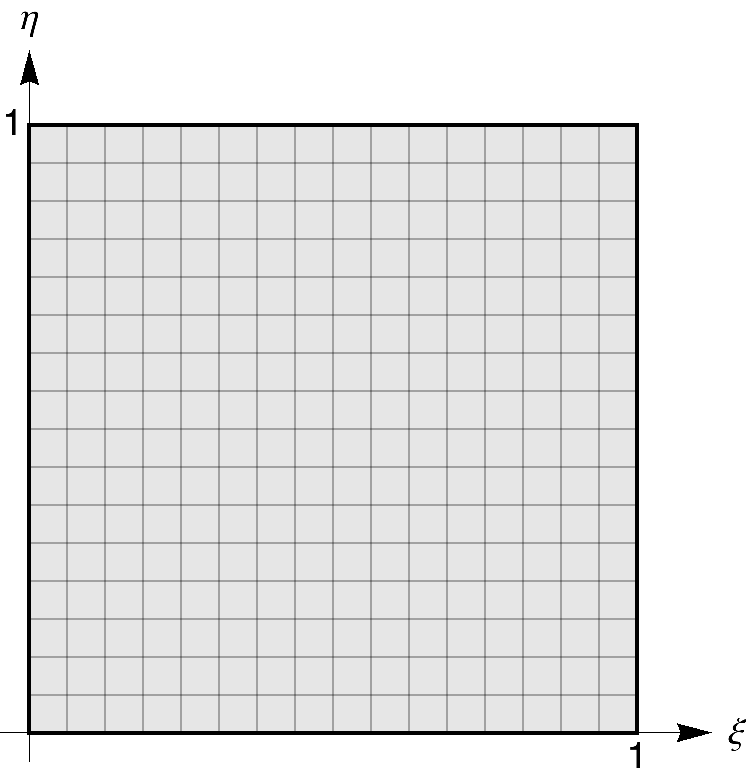
\includegraphics[width=.45\textwidth]{fig/testfig2.pdf}}
\caption{Figure Captions.}
\label{fig:label}
\end{figure}

\end{section}



%=== Appendix ============================================
\appendix

\dsp

\chapter{Appendix Title }{\label{appendix:a}}
\begin{section}{Section Title}

Appendicitis

\end{section}
\end{mainmatter}

%----- Bibliography ----------------
\ssp
\bibliographystyle{JHEP3}
\bibliography{dissertation}

\end{document} 
